% Created by tikzDevice version 0.12.6 on 2026-08-03 04:28:26
% !TEX encoding = UTF-8 Unicode
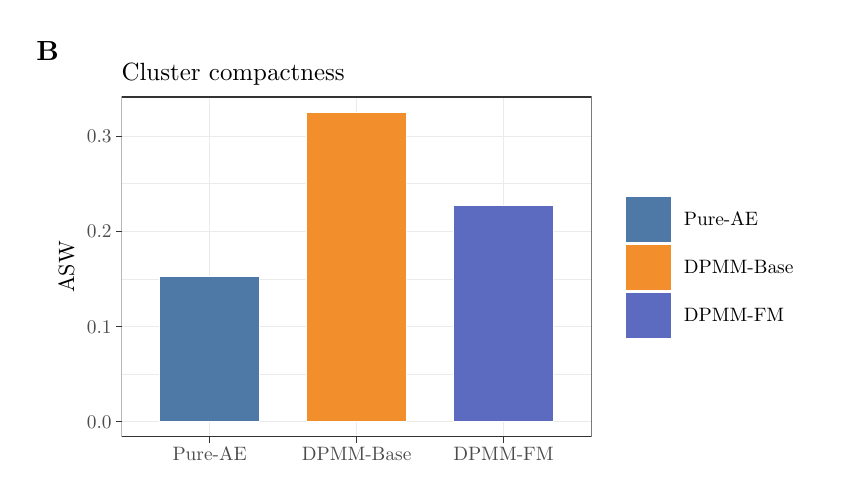
\begin{tikzpicture}[x=1pt,y=1pt]
\definecolor{fillColor}{RGB}{255,255,255}
\path[use as bounding box,fill=fillColor,fill opacity=0.00] (0,0) rectangle (285.80,161.83);
\begin{scope}
\path[clip] (  1.11,  1.74) rectangle (284.69,160.09);
\definecolor{drawColor}{RGB}{255,255,255}
\definecolor{fillColor}{RGB}{255,255,255}

\path[draw=drawColor,line width= 0.4pt,line join=round,line cap=round,fill=fillColor] (  1.11,  1.74) rectangle (284.69,160.09);
\end{scope}
\begin{scope}
\path[clip] ( 33.93, 13.93) rectangle (203.76,136.79);
\definecolor{fillColor}{RGB}{255,255,255}

\path[fill=fillColor] ( 33.93, 13.93) rectangle (203.76,136.79);
\definecolor{drawColor}{gray}{0.92}

\path[draw=drawColor,line width= 0.2pt,line join=round] ( 33.93, 36.70) --
	(203.76, 36.70);

\path[draw=drawColor,line width= 0.2pt,line join=round] ( 33.93, 71.07) --
	(203.76, 71.07);

\path[draw=drawColor,line width= 0.2pt,line join=round] ( 33.93,105.44) --
	(203.76,105.44);

\path[draw=drawColor,line width= 0.4pt,line join=round] ( 33.93, 19.52) --
	(203.76, 19.52);

\path[draw=drawColor,line width= 0.4pt,line join=round] ( 33.93, 53.89) --
	(203.76, 53.89);

\path[draw=drawColor,line width= 0.4pt,line join=round] ( 33.93, 88.26) --
	(203.76, 88.26);

\path[draw=drawColor,line width= 0.4pt,line join=round] ( 33.93,122.63) --
	(203.76,122.63);

\path[draw=drawColor,line width= 0.4pt,line join=round] ( 65.77, 13.93) --
	( 65.77,136.79);

\path[draw=drawColor,line width= 0.4pt,line join=round] (118.85, 13.93) --
	(118.85,136.79);

\path[draw=drawColor,line width= 0.4pt,line join=round] (171.92, 13.93) --
	(171.92,136.79);
\definecolor{drawColor}{RGB}{255,255,255}
\definecolor{fillColor}{RGB}{242,142,43}

\path[draw=drawColor,line width= 0.3pt,fill=fillColor] (100.80, 19.52) rectangle (136.89,131.21);
\definecolor{fillColor}{RGB}{92,107,192}

\path[draw=drawColor,line width= 0.3pt,fill=fillColor] (153.87, 19.52) rectangle (189.96, 97.56);
\definecolor{fillColor}{RGB}{78,121,167}

\path[draw=drawColor,line width= 0.3pt,fill=fillColor] ( 47.73, 19.52) rectangle ( 83.82, 71.81);
\definecolor{drawColor}{gray}{0.20}

\path[draw=drawColor,line width= 0.4pt,line join=round,line cap=round] ( 33.93, 13.93) rectangle (203.76,136.79);
\end{scope}
\begin{scope}
\path[clip] (  0.00,  0.00) rectangle (285.80,161.83);
\definecolor{drawColor}{gray}{0.30}

\node[text=drawColor,anchor=base east,inner sep=0pt, outer sep=0pt, scale=  0.70] at ( 30.33, 17.11) {0.0};

\node[text=drawColor,anchor=base east,inner sep=0pt, outer sep=0pt, scale=  0.70] at ( 30.33, 51.48) {0.1};

\node[text=drawColor,anchor=base east,inner sep=0pt, outer sep=0pt, scale=  0.70] at ( 30.33, 85.85) {0.2};

\node[text=drawColor,anchor=base east,inner sep=0pt, outer sep=0pt, scale=  0.70] at ( 30.33,120.22) {0.3};
\end{scope}
\begin{scope}
\path[clip] (  0.00,  0.00) rectangle (285.80,161.83);
\definecolor{drawColor}{gray}{0.20}

\path[draw=drawColor,line width= 0.4pt,line join=round] ( 31.93, 19.52) --
	( 33.93, 19.52);

\path[draw=drawColor,line width= 0.4pt,line join=round] ( 31.93, 53.89) --
	( 33.93, 53.89);

\path[draw=drawColor,line width= 0.4pt,line join=round] ( 31.93, 88.26) --
	( 33.93, 88.26);

\path[draw=drawColor,line width= 0.4pt,line join=round] ( 31.93,122.63) --
	( 33.93,122.63);
\end{scope}
\begin{scope}
\path[clip] (  0.00,  0.00) rectangle (285.80,161.83);
\definecolor{drawColor}{gray}{0.20}

\path[draw=drawColor,line width= 0.4pt,line join=round] ( 65.77, 11.93) --
	( 65.77, 13.93);

\path[draw=drawColor,line width= 0.4pt,line join=round] (118.85, 11.93) --
	(118.85, 13.93);

\path[draw=drawColor,line width= 0.4pt,line join=round] (171.92, 11.93) --
	(171.92, 13.93);
\end{scope}
\begin{scope}
\path[clip] (  0.00,  0.00) rectangle (285.80,161.83);
\definecolor{drawColor}{gray}{0.30}

\node[text=drawColor,anchor=base,inner sep=0pt, outer sep=0pt, scale=  0.70] at ( 65.77,  5.51) {Pure-AE};

\node[text=drawColor,anchor=base,inner sep=0pt, outer sep=0pt, scale=  0.70] at (118.85,  5.51) {DPMM-Base};

\node[text=drawColor,anchor=base,inner sep=0pt, outer sep=0pt, scale=  0.70] at (171.92,  5.51) {DPMM-FM};
\end{scope}
\begin{scope}
\path[clip] (  0.00,  0.00) rectangle (285.80,161.83);
\definecolor{drawColor}{RGB}{0,0,0}

\node[text=drawColor,rotate= 90.00,anchor=base,inner sep=0pt, outer sep=0pt, scale=  0.80] at ( 16.80, 75.36) {ASW};
\end{scope}
\begin{scope}
\path[clip] (  0.00,  0.00) rectangle (285.80,161.83);
\definecolor{fillColor}{RGB}{255,255,255}

\path[fill=fillColor] (211.76, 45.35) rectangle (282.69,105.38);
\end{scope}
\begin{scope}
\path[clip] (  0.00,  0.00) rectangle (285.80,161.83);
\definecolor{fillColor}{RGB}{255,255,255}

\path[fill=fillColor] (215.76, 84.03) rectangle (233.11,101.38);
\definecolor{drawColor}{RGB}{255,255,255}
\definecolor{fillColor}{RGB}{78,121,167}

\path[draw=drawColor,line width= 0.3pt,fill=fillColor] (216.12, 84.39) rectangle (232.75,101.02);
\end{scope}
\begin{scope}
\path[clip] (  0.00,  0.00) rectangle (285.80,161.83);
\definecolor{fillColor}{RGB}{255,255,255}

\path[fill=fillColor] (215.76, 66.69) rectangle (233.11, 84.03);
\definecolor{drawColor}{RGB}{255,255,255}
\definecolor{fillColor}{RGB}{242,142,43}

\path[draw=drawColor,line width= 0.3pt,fill=fillColor] (216.12, 67.05) rectangle (232.75, 83.68);
\end{scope}
\begin{scope}
\path[clip] (  0.00,  0.00) rectangle (285.80,161.83);
\definecolor{fillColor}{RGB}{255,255,255}

\path[fill=fillColor] (215.76, 49.35) rectangle (233.11, 66.69);
\definecolor{drawColor}{RGB}{255,255,255}
\definecolor{fillColor}{RGB}{92,107,192}

\path[draw=drawColor,line width= 0.3pt,fill=fillColor] (216.12, 49.70) rectangle (232.75, 66.33);
\end{scope}
\begin{scope}
\path[clip] (  0.00,  0.00) rectangle (285.80,161.83);
\definecolor{drawColor}{RGB}{0,0,0}

\node[text=drawColor,anchor=base west,inner sep=0pt, outer sep=0pt, scale=  0.70] at (237.11, 90.30) {Pure-AE};
\end{scope}
\begin{scope}
\path[clip] (  0.00,  0.00) rectangle (285.80,161.83);
\definecolor{drawColor}{RGB}{0,0,0}

\node[text=drawColor,anchor=base west,inner sep=0pt, outer sep=0pt, scale=  0.70] at (237.11, 72.95) {DPMM-Base};
\end{scope}
\begin{scope}
\path[clip] (  0.00,  0.00) rectangle (285.80,161.83);
\definecolor{drawColor}{RGB}{0,0,0}

\node[text=drawColor,anchor=base west,inner sep=0pt, outer sep=0pt, scale=  0.70] at (237.11, 55.61) {DPMM-FM};
\end{scope}
\begin{scope}
\path[clip] (  0.00,  0.00) rectangle (285.80,161.83);
\definecolor{drawColor}{RGB}{0,0,0}

\node[text=drawColor,anchor=base west,inner sep=0pt, outer sep=0pt, scale=  0.90] at ( 33.93,142.78) {Cluster compactness};
\end{scope}
\begin{scope}
\path[clip] (  0.00,  0.00) rectangle (285.80,161.83);
\definecolor{drawColor}{RGB}{0,0,0}

\node[text=drawColor,anchor=base,inner sep=0pt, outer sep=0pt, scale=  1.00] at (  7.20,150.08) {\bfseries B};
\end{scope}
\end{tikzpicture}
